\begin{document}

\frontmatter
\maketitle
\makeabstract
\tableofcontents
\listoffigures
\listoftables
\mainmatter

\chapter{基本格式测试}\label{chapter:1}

\section{第一层}\label{sec:1}
\subsection{第二层}\label{sec:2}
\subsubsection{第三层}\label{sec:3}
测试测试测试测试测试测试测试测试测试测试测试测试。
\footnote{\label{footnote:1}脚注}

\section{字体}

普通\textbf{粗体}\emph{斜体}

\hei{黑体}\kai{楷体}\fangsong{仿宋}

\section{公式}

单个公式,公式引用:\autoref{eq:1}。
\begin{equation}
 c^2 = a^2 + b^2 \label{eq:1}
\end{equation}

多个公式,公式引用:\autoref{eq:2},\autoref{eq:3}。

\begin{subequations}
\begin{equation}
  F = ma \label{eq:2}
\end{equation}
\begin{equation}
  E = mc^2 \label{eq:3}
\end{equation}
\end{subequations}

\section{罗列环境}

\begin{enumerate}
    \item 第一层\label{item:1}
    \item 第一层
    \begin{enumerate}
        \item 第二层\label{item:2}
        \item 第二层
        \begin{enumerate}
            \item 第三层\label{item:3}
            \item 第三层
        \end{enumerate}
    \end{enumerate}
\end{enumerate}

\begin{description}
    \item[解释环境]  解释内容
\end{description}

\chapter{其他格式测试}

\section{代码环境}

\begin{lstlisting}[language=python]
import os

def main():
    '''
    doc here
    '''
    print 'hello, world' # Abc
    print 'hello, 中文' # 中文
\end{lstlisting}

\section{定律证明环境}

\begin{definition}\label{def:1}
这是一个定义。
\end{definition}
\begin{proposition}\label{proposition:1}
这是一个命题。
\end{proposition}
\begin{axiom}\label{axiom:1}
这是一个公理。
\end{axiom}
\begin{lemma}\label{lemma:1}
这是一个引理。
\end{lemma}
\begin{theorem}\label{theorem:1}
这是一个定理。
\end{theorem}
\begin{proof}\label{proof:1}
这是一个证明。
\end{proof}

\section{算法环境}

\begin{algorithm}[H]
\SetAlgoLined
\KwData{this text}
\KwResult{how to write algorithm with \LaTeX2e }
initialization\;\label{alg_line:1}
\While{not at end of this document}{
read current\;
\eIf{understand}{
go to next section\;
current section becomes this one\;
}{
go back to the beginning of current section\;
}
}
\caption{How to write algorithms}\label{alg:1}
\end{algorithm}

\section{表格}
表格见\autoref{tab:1}。

\begin{table}[!h]
\centering
\caption{一个表格}\label{tab:1}
\begin{tabular}{|c|c|}
\hline
a & b \\
\hline
c & d \\
\hline
\end{tabular}
\end{table}
\section{图片}
图片见\autoref{fig:1}。图片格式支持eps,png,pdf等。多个图片见\autoref{fig:2},分开引用:\autoref{fig:2-1},\autoref{fig:2-2}。

\begin{figure}[!h]
\centering
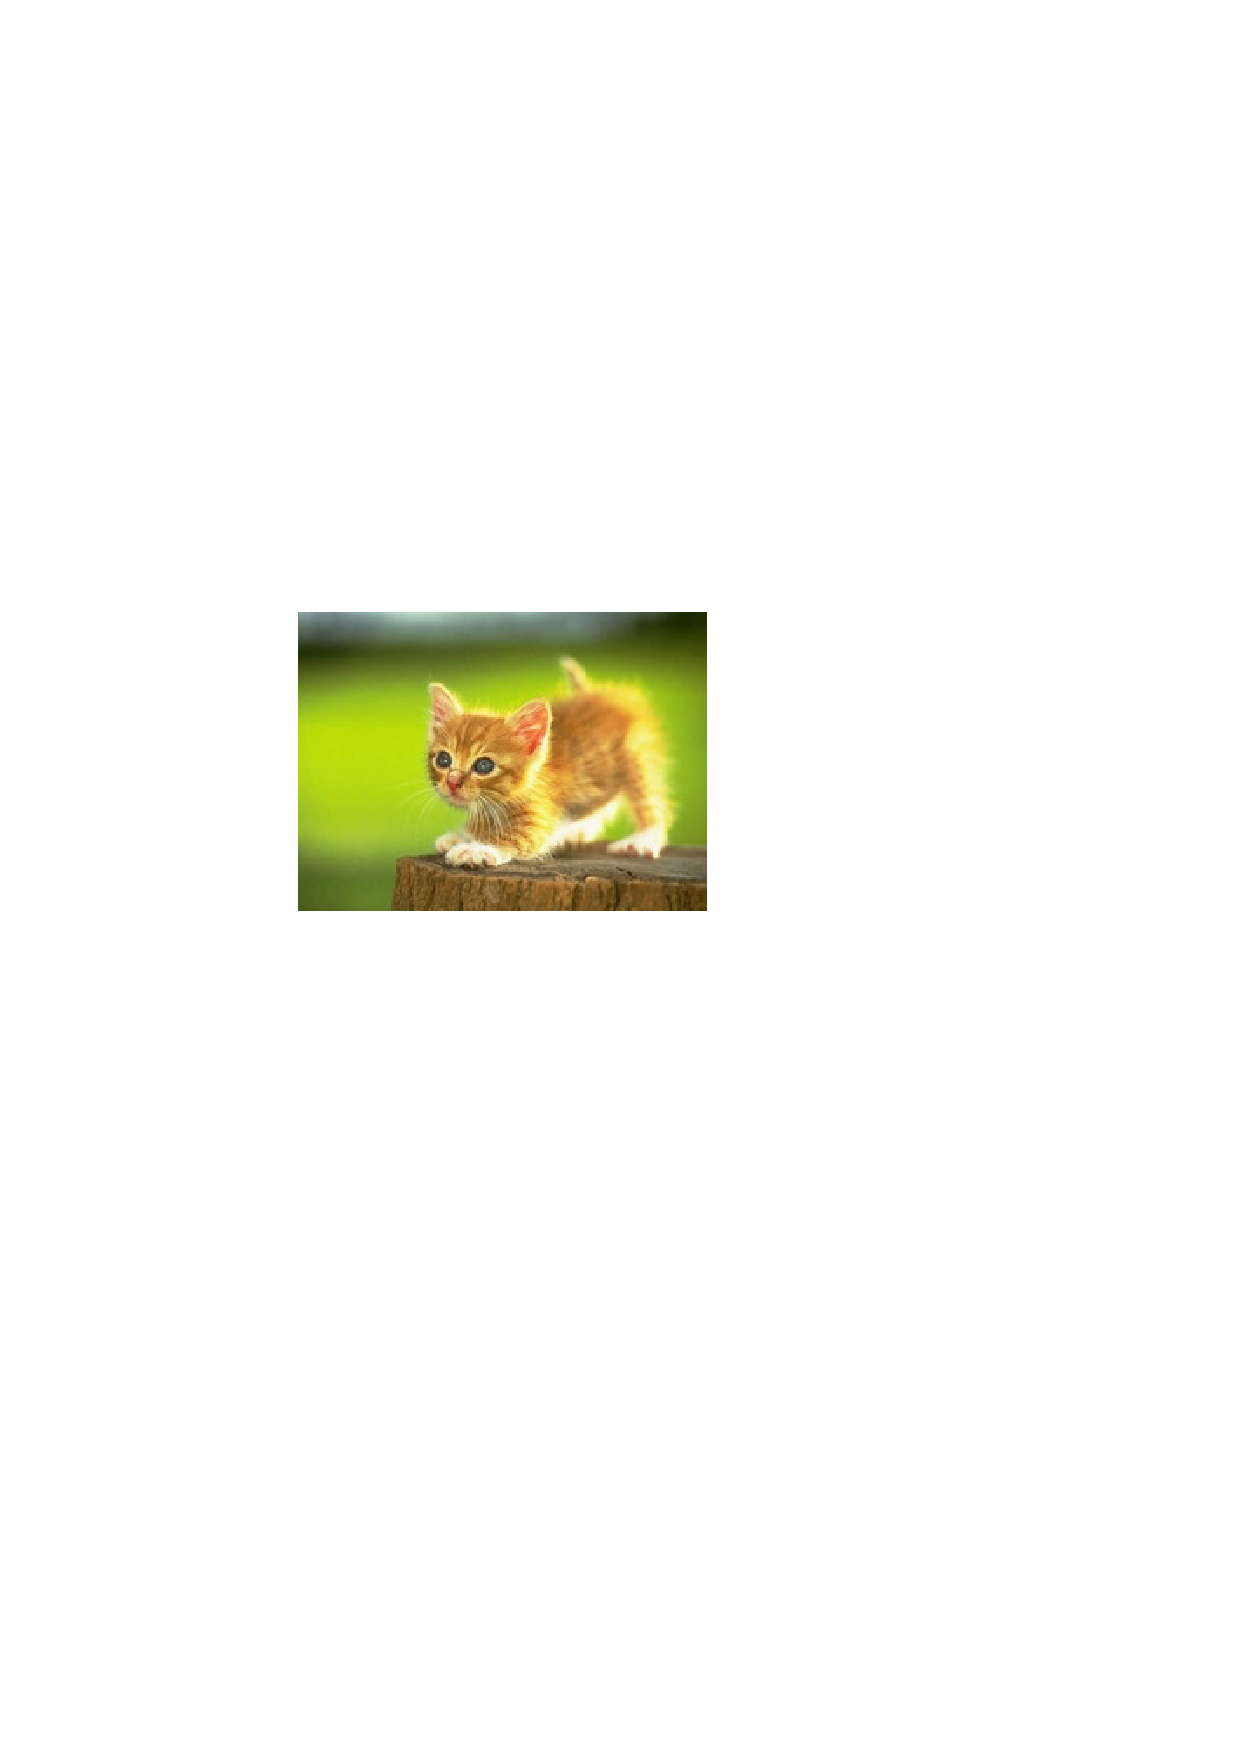
\includegraphics[width=.4\textwidth]{fig-example.pdf}
\caption{一个图片}\label{fig:1}
\end{figure}

\begin{figure}[!h]
\centering
  \begin{subfigure}[b]{0.3\textwidth}
  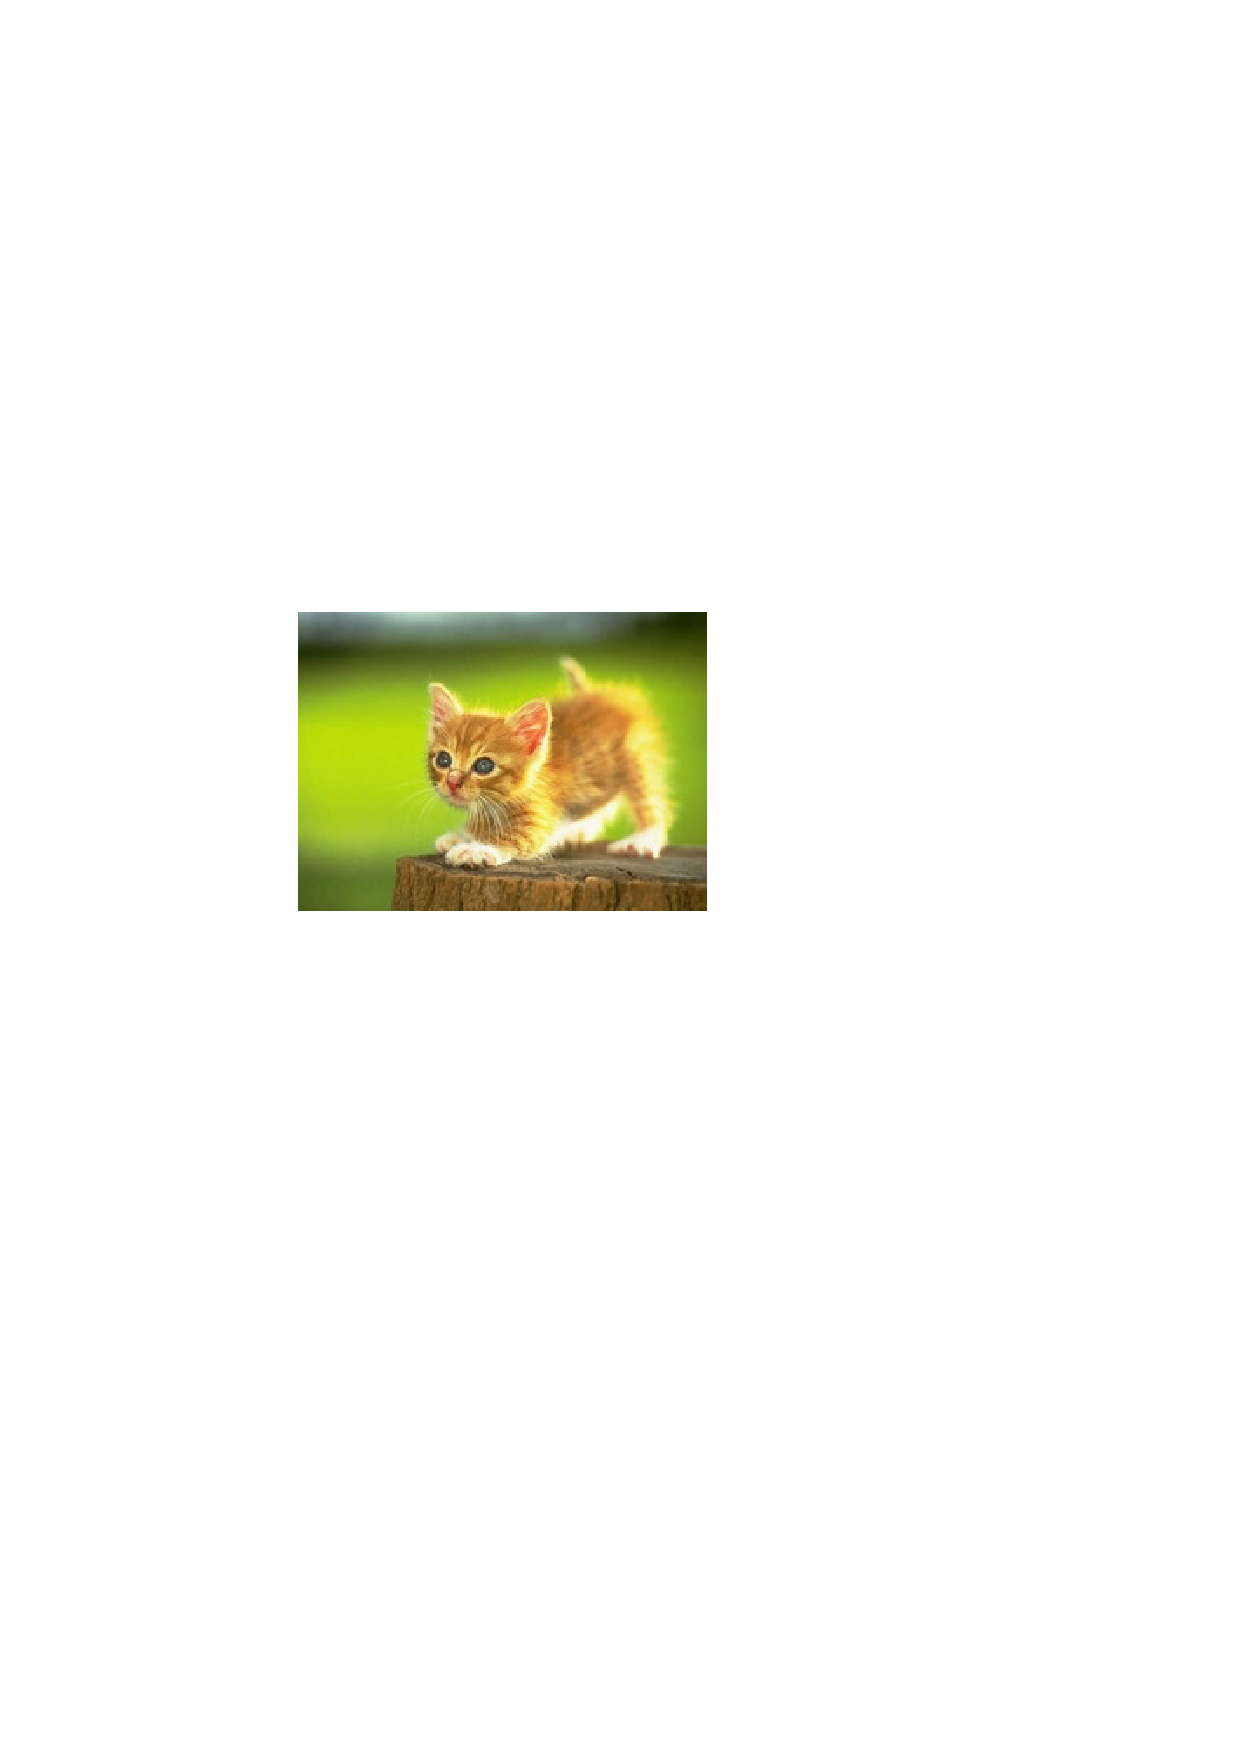
\includegraphics[width=\textwidth]{fig-example.pdf}
  \caption{图片1}\label{fig:2-1}
  \end{subfigure}
  ~
  \begin{subfigure}[b]{0.3\textwidth}
  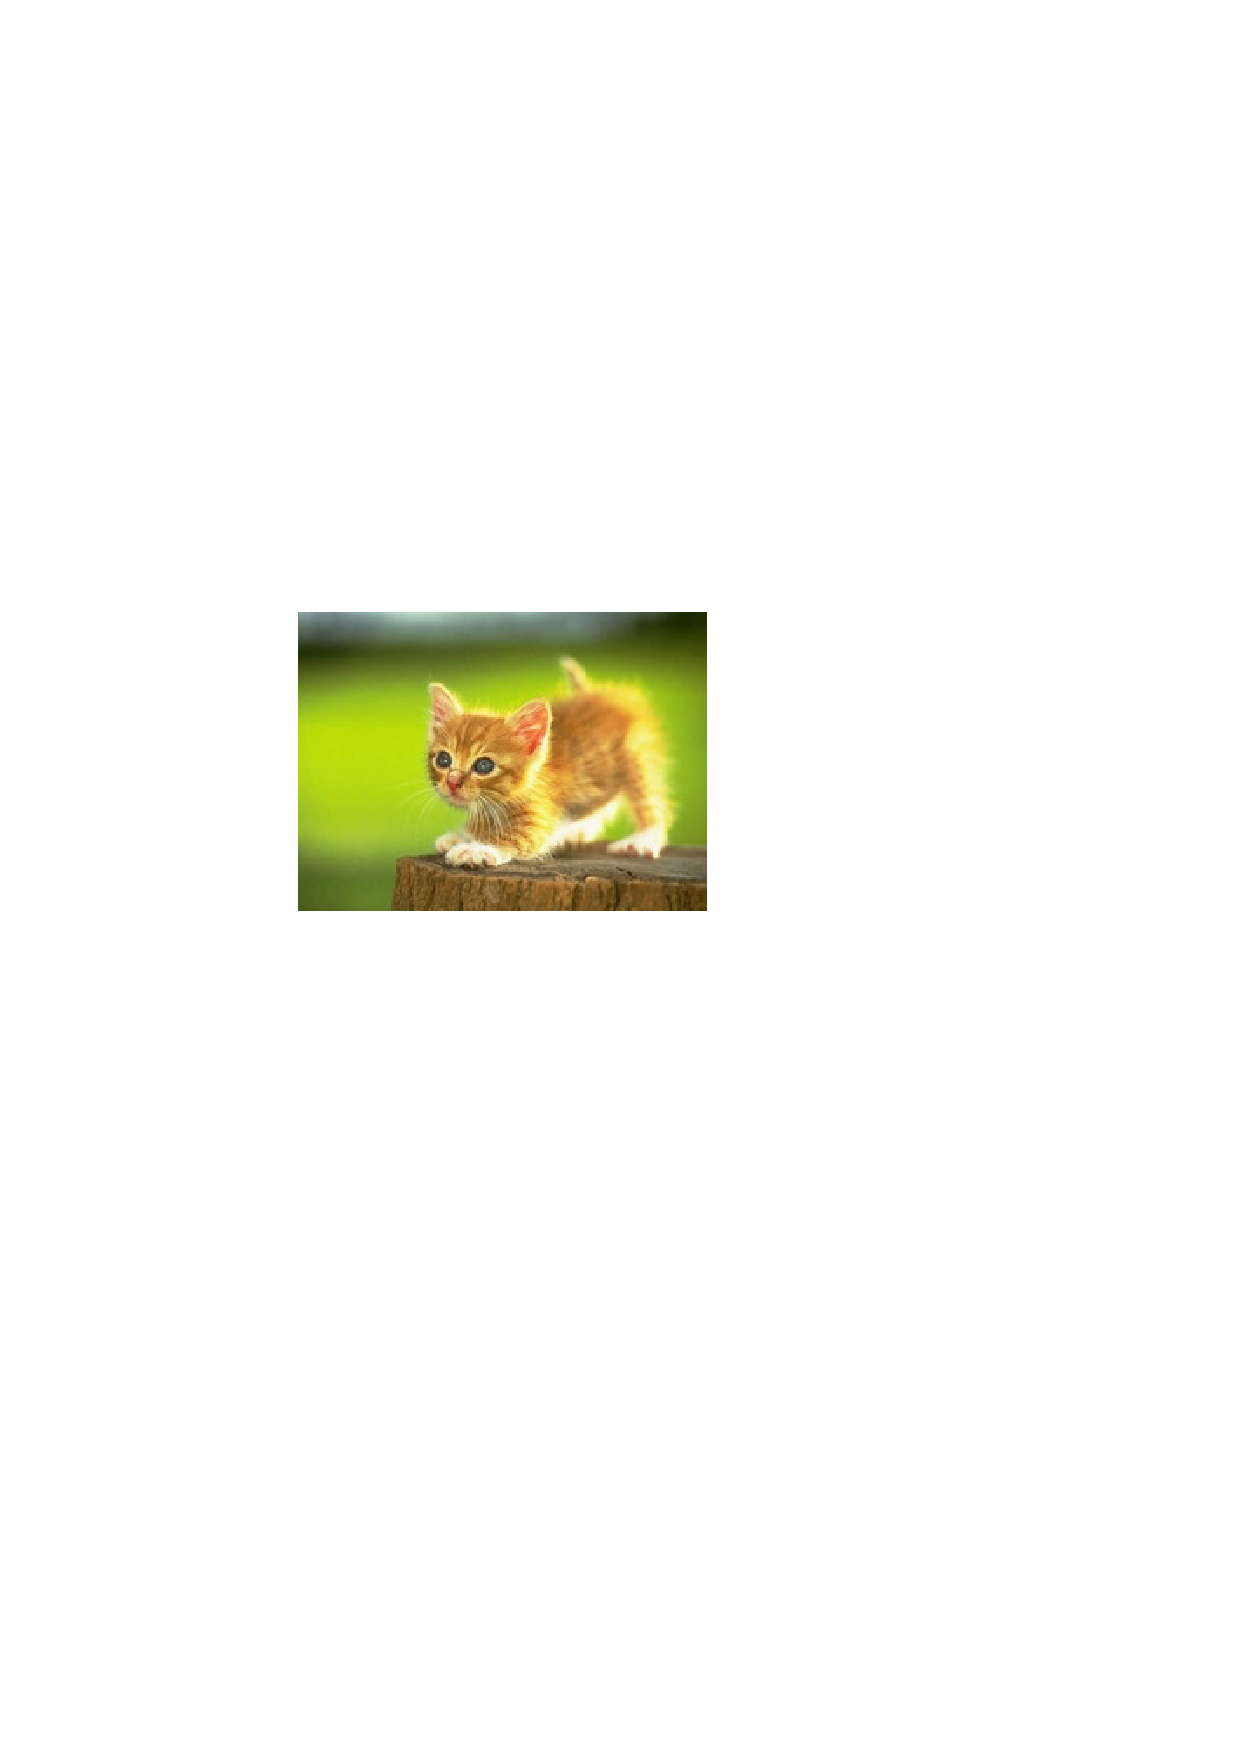
\includegraphics[width=\textwidth]{fig-example.pdf}
  \caption{图片2}\label{fig:2-2}
  \end{subfigure}
\caption{多个图片}\label{fig:2}
\end{figure}

\section{参考文献示例}
这是一篇中文参考文献\cite{TEXGURU99};这是一篇英文参考文献\cite{knuth};同时引用\cite{TEXGURU99,knuth}。

\section[\textbackslash{}autoref 测试]{\texttt{\textbackslash{}autoref} 测试}

\begin{description}
  \item[公式] \autoref{eq:1}
  \item[脚注] \autoref{footnote:1}
  \item[项] \autoref{item:1},\autoref{item:2},\autoref{item:3}
  \item[图] \autoref{fig:1}
  \item[表] \autoref{tab:1}
  \item[附录] \autoref{appendix:1}
  \item[章] \autoref{chapter:1}
  \item[小节] \autoref{sec:1},\autoref{sec:2},\autoref{sec:3}
  \item[算法] \autoref{alg:1},\autoref{alg_line:1}
  \item[证明环境] \autoref{def:1},\autoref{proposition:1},\autoref{axiom:1},\autoref{lemma:1},\autoref{theorem:1},\autoref{proof:1}
\end{description}

\backmatter

\begin{ack}
致谢正文。
\end{ack}

\bibliography{ref-example}

\appendix

\begin{publications}
    \item 论文1
    \item 论文2
\end{publications}

\chapter{这是一个附录}\label{appendix:1}
附录正文。


\end{document}
\endinput
%%
%% End of file `hustthesis-zh-example.tex'.







校研[2005] 51号



学位论文是学位申请人为申请学位而撰写的学术论文,是评判学位申请人学术水平的重要依据和获得学位的必要条件,也是科研领域中的重要文献资料和社会的宝贵财富。为进一步提高我校博士、硕士学位论文的质量,规范学位论文格式,特作如下规定。

一、基本要求
1.硕士学位论文应能表明作者确已在本门学科上掌握了坚实的基础理论和系统的专门知识,并对所研究课题有新的见解,有从事科学研究工作或独立担负专门技术工作的能力。

2.博士学位论文应能表明作者确已在本门学科上掌握了坚实宽广的基础理论和系统深入的专门知识,并具有独立从事科学研究工作的能力,在科学或专门技术上做出了创造性的成果。

3.学位论文一般应用中文撰写,硕士学位论文正文应不少于2万字,博士学位论文正文要求5-8万字。学位论文内容应立论正确、推理严谨、文字简练、层次分明、说理透彻、数据真实可靠。

4.论文作者应在选题前后阅读有关文献,硕士学位申请人的文献阅读量不少于40篇,其中外文文献至少应占三分之一;博士学位申请人的文献阅读量不少于60篇,其中外文文献至少应占三分之二。综述部分应对所读文献加以分析和综合。

5.量和单位及其符号均应符合国家标准的规定,国家标准中未规定的,应执行国际标准或行业标准;不同的量必须用不同的符号表示,不得一符多义,含义相同的量则必须用同一符号表示。学位论文应用最新颁布的汉语简化文字,符合《出版物汉字使用管理规定》;专业术语应统一使用全国自然科学名词审定委员会公布的各学科名词,或本学科权威专着和期刊通用的专业术语,且前后应一致;标点符号的使用应符合国家标准《标点符号用法》的规定;数字的使用应符合国家标准《出版物上数字用法的规定》。

6.图要精选,切忌与文字或表内容重复,图中文字、数据和符号应准确无误且与文字叙述一致,图应有图号和图名,图名应简洁明确且与图中内容相符。表应有表序和表名,表名应简洁并与内容相符。图、表和公式应分别顺序编号。

二、题名
题名是以最恰当、最简明的词语反映论文中最重要的特定内容的逻辑组合。题名既要准确地描述内容,又要尽可能地精练,一般不宜超过20个字。题名应该避免使用不常见的缩略词、字符、代号和公式等。外文题名一般不宜超过10个实词。

三、序或前言(必要时)
序或前言一般是作者对学位论文基本特征的简介,如说明选题的缘起、背景、主旨、目的、意义,以及资助、支持、协作经过等;也可以评述和对相关问题的研究进行说明。序或前言并非必需。这些内容也可以在正文引言中和致谢中陈述。

四、摘要和关键词
摘要是学位论文极为重要、不可缺少的组成部分,它是论文的窗口,并频繁用于国内外资料交流、情报检索、二次文献编辑等。其性质和要求如下:

1.摘要即摘录论文要点,是论文要点不加注释和评论的一篇完整的陈述性短文,具有很强的自含性和独立性,能独立使用和被引用。

2.应含有学位论文全文的主要信息,硕士学位论文摘要应突出新见解与成果,博士学位论文摘要应突出创造性成果。

3.内容范围应包含以下基本要素:

(1)目的:研究、研制、调查等的前提、目的和任务以及所涉及的主题范围。

(2)方法:所用原理、理论、条件、对象、材料、工艺、手段、装备、程序等。

(3)结果:实验的、研究的、调查的、观察的结果、数据,被确定的关系,得到的效果、性能等。

(4)结论:结果的分析、研究、比较、评价、应用;提出的问题,今后的课题,建议,预测等。

(5)其他:不属于研究、研制、调查的主要目的,但就其见识和情报价值而言也是重要的信息。

4.摘要的详简度视论文的内容、性质而定,硕士学位论文摘要一般为500-600汉字,博士学位论文摘要一般为800-1000汉字。

5.摘要中一般不用图、表、化学结构式、计算机程序,不用非公知公用的符号、术语和非法定的计量单位。

6.关键词应有3至8个,另起一行置于摘要下方。涉及的内容、领域从大到小排列,便于文献编目与查询。

7.应有与中文摘要和关键词相对应的英文摘要和关键词。英语摘要用词应准确,使用本学科通用的词汇;摘要中主语(作用)常常省略,因而一般使用被动语态;应使用正确的时态,并要注意主、谓语的一致,必要的冠词不能省略。

五、引言或绪论
引言或绪论应简要说明研究工作的目的、范围、相关领域的前人工作和知识空白、理论基础和分析、研究设想、研究方法和实验设计、预期结果和意义等。

六、正文
正文是核心部分,占主要篇幅,可以包括:研究对象、理论模型、实验和观测方法、仪器设备、材料原料、实验和观测结果、计算方法和编程原理、数据资料、经过加工整理的图表、形成的论点和导出的结论等。各章节标题应大致对称,内容之间有严密的逻辑论证关系,各部分篇幅长短不宜悬殊太大,章节标题也不宜太长。

由于研究工作涉及的学科、选题、研究方法、工作进程、结果表达方式等有很大的差异,对正文内容不作统一的规定。但是,必须实事求是,客观真切,准确完备,合乎逻辑,层次分明,简练可读。

七、结论
经过对实验记录和实验结果等的综合分析研究,归纳出若干有机联系的论点,并对本研究成果的意义、推广应用的现实性或可能性和进一步发展的探讨加以论述。结论应该准确、完整、明确、精练。

如果不可能导出应有的结论,也可以没有结论而进行必要的讨论。

八、致谢
对在完成课题研究和论文写作过程中给予指导和帮助的导师、校内外专家、实验技术人员、同学等表示感谢。

九、参考文献
在论文中引用了文献内容的,应将其列入参考文献表。

1.参考文献标注法,在正文中引用文献内容处注明参考文献编号。参考文献目录按正文中引用先后顺序排列,重复引用的文献,按第一次出现的顺序编号。

2.文科论文参考文献标注法,可按国际惯例,英文文献用作者姓氏和发表年份加上圆括号来标注,例如(Farrell,1997);中文文献用作者姓名和发表年份加上圆括号来标注,例如(张华,2000)。当文献作者有两个时,标注方式如(Sommerset and Lovekin,2000)或(张华,李平,2000)。当文献作者多于两个时,标注方式如(Sommerset et al,2000)或(李平等,2000)。如果同一作者有一个以上同一年份的文献被引用,那么在文献标注和参考文献目录中要增加一个标识符,如(1985a),(1985b)。如果论文中已经提到了作者姓名,则只需在作者姓名后面用发表年份加圆括号标注,例如“ F.Modigliani(1960)指出……” 。参考文献目录按姓氏或姓氏汉语拼音的字母顺序排列,汉字姓名以姓氏汉语拼音字母为序,英语姓名以姓氏字母为序。

3.可列于参考文献表的文献类型包括图书、期刊、会议论文集、专利和学位论文等。其著录格式分别如下(注意标点符号):

(1) 图书:[顺序编号] 作者(采用姓在前,名在后的形式,作者名之间用逗号分隔;3人以内全部写上,3人以上只写3人再加“等”(英文加“ et al”)).书名.版本(第×版).译者.出版地:出版者,出版年.起页~止页

(2) 期刊:[顺序编号] 作者(采用姓在前,名在后的形式,作者名之间用逗号分隔;3人以内全部写上,3人以上只写3人再加“等”(英文加“ et al”)).文章名称.期刊名称,年号,卷号(期号):起页~止页

(3) 会议论文集:[顺序编号] 作者(采用姓在前,名在后的形式,作者名之间用逗号分隔;3人以内全部写上,3人以上只写3人再加“等”(英文加“ et al”)).文章名称.见(英文用“in”):论文集主编.论文集名.出版地:出版者,出版年.起页~止页

(4) 专利:[顺序编号] 专利申请者.专利题名.专利国别,专利文献种类,专利号,出版年.起页~止页

(5) 学位论文:[顺序编号] 作者.题名:[博士(或硕士)学位论文]。保存地点:保存单位(如华中科技大学图书馆),年份.

4.当论文中有些术语、公式、背景或数据来源需要解释或说明,以及援引他人的原话、数据等资料而必须指明资料来源时,可用脚注。脚注要按顺序编号。脚注按每一页单独编号。脚注的标识可以用数字1,2等,也可以用符号① ,②等。脚注的资料来源表示方法同参考文献。

十、附录(必要时)
包括详细的公式推导、实验数据、计算程序、援引他人的原始资料、数据及其设备条件等。

学位申请人攻读学位期间发表的学术论文目录置于附录1,格式同第九条要求,并逐篇注明署名单位是否为华中科技大学。

十一、编排格式要求
1. 学位论文封面内容与格式由研究生院统一规定。封面上“分类号”和“密级”一般不填,保密的论文按照校保密办认定的密级填写;学校代码为10487;“指导教师”栏可填正、副导师。

2. 论文外形尺寸以A4本为准。装订顺序为:封面、英文扉页、独创性声明和学位论文版权使用授权书、序或前言(必要时)、中文摘要和关键词、英文摘要和关键词、目次页、引言、正文、结论、致谢、参考文献、附录(必要时)、封三、封四。

3. 学位论文文字排版的字号、行距、字距的大小,以版面清晰、容易辨识和阅读为原则,一般可参照下面要求进行排版:章和节的题名用黑体,字号分别用3号和4号;文章段落内容用小四号宋体字,行间距不小于三分之二字高度;正文中标题一律左顶格。正文编排式样见附件1。

4. 目次页编排式样见附件2。

十二、本规定自公布之日起施行,由研究生院负责解释。